    \subsection*{Choice of $k$}
    
        One important question we decided to \textbf{ignore} earlier was: \textbf{how many} clusters should we pick in advance?
        
        Especially for \textbf{complex} data, we \textbf{don't know} how many natural clusters there will be. 
        
        But our number of clusters matter: because it's a parameter determines \textbf{how} our learning algorithm runs (rather than being chosen \textit{by} the algorithm), it's a \textbf{hyperparameter}:\\
        
        \begin{concept}
            Our \vocab{number of clusters} $k$ is a \vocab{hyperparameter}.
        \end{concept}
        
        And, choosing too high \textit{or} too low can both be \textbf{problematic}:
        
        \begin{itemize}
            \item If we set $k$ too \textbf{high}, then we have more clusters than actually \textbf{exist}.
                \begin{itemize}
                    \item This can cause us to \textbf{split} real clusters in half, or find \textbf{patterns} that don't exist.
                    
                    \item In a way, this resembles a kind of \textbf{overfitting}: we try to \textbf{closely} match the data, but end up fitting \textbf{too closely} and not \textbf{generalizing} well: \textbf{estimation error}.
                    
                    \item \miniex The \textbf{extreme} case looks like the example we mentioned \textbf{before}: when labeling animals, we could make... a different \textbf{species} for every single instance of \textbf{any} animal we find. 
                        \note{That doesn't sound very helpful.}
                \end{itemize}
            \item If we set $k$ too \textbf{low}, we don't have \textbf{enough} clusters to represent our data.
                \begin{itemize}
                    \item This means some clusters will be \textbf{lumped together} as a single thing: we \textbf{lose} some information.
                    
                    \item In this case, it's \textbf{impossible} to cluster everything in the way that would make the most \textbf{sense}: we have \textbf{structural error}.
                    
                    \item \miniex Let's say we wanted to \textbf{sort} fish, birds, and mammals into \textbf{two} categories: we might just \textbf{divide} them into "flies" and "doesn't fly".
                        \note{That's some information, but often not enough!}\\
                \end{itemize}
        \end{itemize}
        
        \begin{concept}
            When choosing $k$ (our \vocab{number of clusters}), we can cause \purp{problems} by picking an inappropriate \gren{value}:
            
            \begin{itemize}
                \item \vocab{Too many} clusters (large $k$) can cause \gren{overfitting} and \purp{estimation error}: we find patterns we don't want.
                
                \item \vocab{Not enough} clusters (small $k$) causes \purp{structural error}: it prevents us from correctly \gren{separating} data.
            \end{itemize}
        \end{concept}
        
    \subsection*{Subjectivity of $k$}
    
        Not only is it hard to choose a "good" value of $k$, what a good value of $k$ is can really depend on your opinion, and what you know about reality.
        
        For example, consider the following example:
        
        \begin{figure}[H]
            \centering
            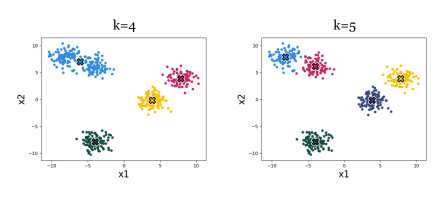
\includegraphics[width=100mm,scale=0.4]{images/clustering_images/subjective_k_value.png}
            \caption*{Which of these two clusterings is more accurate?}
        \end{figure}
        
        Should the top left be \textbf{one} cluster, or \textbf{two}? It's hard to say!
        
        Even if you're \textbf{sure}, you might \textbf{disagree} with others, or find that the best one depends on your \textbf{needs}.
        
        So not only can $k$ values be too high or too low, they can also be \textbf{debatably} better or worse!
        
        \begin{concept}
            The \vocab{best} choice of \vocab{clustering} is not entirely objective: it can depend on your \gren{opinion}, or how you plan to \purp{use} the clustering.
        \end{concept}
        
        What do we mean by, what we're "\textbf{using}" the clustering for? We'll get into that later, but in short: we might use \textbf{clusters} to make sense of \textbf{information}, or to make better \textbf{decisions}. 
        
        Different clusterings might be good when you want a different kind of understanding.
        
        \miniex The understanding you get from high-level comparisons (plants vs animals vs bacteria) is different from low-level comparison (cats vs dogs).
    